\section{Measuring TLB size}
	\label{sec:tlb}
TLB is one greatest optimization that makes virtual memory to work fast.
Without TLB, each memory reference will have to do more less than twice memory
reference, for actual physical pages associated with, and for the real address
CPU wants to visit. In this section, I try to measure the TLB size on my
machine. The result is not exactly what I expected, and I will try to explain that in the discussion section~\ref{subsec:tlb-discus}

\subsection{Methodology}
To measure the size of TLB, I choose to observe the timing difference on referencing
memory. If the TLB hits, then the reference should be faster than TLB misses
cases. The goal could be achieved if we carefully construct the memory visiting
sequence, then we can find out the thrashing behavior in timing when come to the
point TLB begins to miss. Specifically, if not mentioned, TLB later all
mentions to data TLB.

\subsubsection{Complications}
But correctly measuring TLB size, is not an easy task due to following complications:

\begin{itemize}
\item Hardware cache can interference heavily during the visiting process. To
correctly measure the event, one needs to distinguish the cache miss event and
TLB miss event. Unfortunately, these two events are usually comparable in missing
penalty, and make things complex. Even worse is that caches are usually physical
associated, and the addresses we can provide at userspace are virtual addresses.
For the set associative caches, if their associative sets number are larger than
the number of cache lines per page, then we can not fully control the cache. Due
to the space limitation, if not necessary, I will omit derivations of the
non-experimental conclusions.
\item Hardware can have mechanism that ruins the assumptions about sequential
programming model, like out-of-order instruction retiring, multiple processing
units, and hardware prefetching and so on.
\item Modern CPU can have multiple level of TLB. On my platform, there is two
L1 data TLB for different page sizes, one L1 instruction TLB, and one shared L2
TLB. We need to let level 1 TLB to fail before we can fail level 2 TLB.
\item Difficulties in generating the correct benchmark. The overhead in
language constructs, operating systems interactions, and the compiler's
aggressive optimizations can all become obstacles to obtain the correct results.
\end{itemize}

\subsubsection{Strategy}
To solve the above complications, I carefully construct my sequence to walk on
memory. First thing is to design a pattern to maximize cache hit. One
observation that helps is: level N TLB (N=1,2) usually has less entries than the total
cache line number in level N cache, but its total size is larger than the corresponding
cache. Due to this fact, we can force level N cache to hit, while level N TLB to miss.

This goal can be achieved by visiting exactly one cache line inside each page.
We first allocate sufficient pages, and gradually increase the number of pages
to walk on.  The phase change point in timing would be approximation size of
TLB size. To make cache hit, the stride we use to walk on pages is sum of page
size and cache line size. This ensures we visit a different set of cache lines
in the next page and will maximize the cache utilization. When it goes off the
page boundary, then just rewind to the start of next page and keep on this
procedure. 

This strategy will work for both L1 and L2 TLB. Actually, by maximize the cache
utilization, at the point of L2-TLB miss, we will observe different timing
behaviors. Let's define $C_i$ to be level i cache hit, $T_i$ to be level i
TLB hit, and $C_m$, $T_m$ to be cache and TLB miss correspondingly. Then we
should observe $C_1T_1$, $C_1T_2$, $C_1T_m$, or $C_1T_1$, $C_1T_2$, $C_2T_2$,
$C_2T_m$. There should not have $C_2T_1$, or $C_mT_2$ behavior, so the timing
curve would be monotonically non-decreasing as we enlarge the walking page size.

Since memory references are tiny things to measure, we repeat the memory walk
many times and measure the average.
%At the beginning I enforced each walk to
%make same number of memory reference, but later I found this is wrong so I
%adjusted to use same iterations for each walk. The reason will be discussed
%in~\ref{subsec:tlb-discussion}

\subsection{Implementation}
The implementation is quite tricky. Firstly I manually unrolled innermost loops
of all walking routines, and ensuring they have the least number of
instructions. This can avoid loop overhead to small loops as well as improve
the hit rate of instruction cache. Additionally, all operands are aligned to same
size to avoid size extending. Before walking, the memory should be warmed
several times and evict out dirty data. The last thing then come with the
compiler optimization. In one hand, we can rely on the optimization to reduce
the uncessary memory visit and computation, rather than manually coding
assembly (actually I did this for some very small walk kernels), but on the
other hand we should add some fake "use" to avoid our code being optimzed out.
Also, inline optimization should not be used abusively. Large chunk of inlined
code can hurt the instruction cache, which is unnecessary overhead.

To automate the experiment, I also write code to measure cache size and
associative sets. I reference the paper here~\cite{sigmetrics:cache}. To avoid
the problem of physical not continuous, I resort to huge pages, and then things
become a lot more easier, just capacity probe suffies to find out how many
cache lines and how many associative sets are in each cache. Due to the space limitation, I don't show the detail here. Further information could be found in~\cite{github}.

\begin{figure}[hpb]
\centering
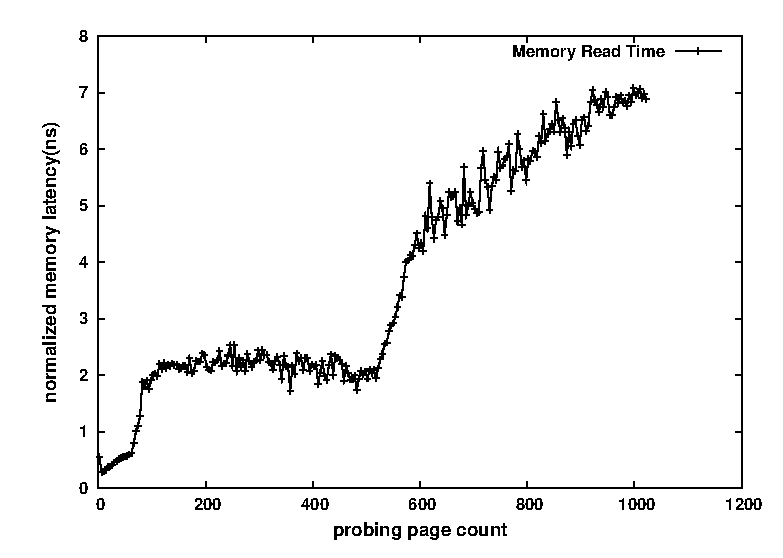
\includegraphics[width=0.9\linewidth]{../figures/time}
\caption{Memory walk time on different number of pages. The stride size I use is 4160 byte, the sum of page size and cache line size, so the memory reference will happen on each page exactly once.}
\label{fig:tlbsz-time}
\end{figure}

\subsection{Experiment Results}

%
%
% 1. cache measuring result
% 2. TLB size measuring result
% 3. huge tlb result
% 4. TLB way measuring
%
%
Figure~\ref{fig:tlbsz-time} shows the timing result of TLB probing. The first
part of the result looks quite reasonable, clear boundary and much stable
than the second half after I have probed about 512 pages.

\begin{figure}[hpb]
\centering
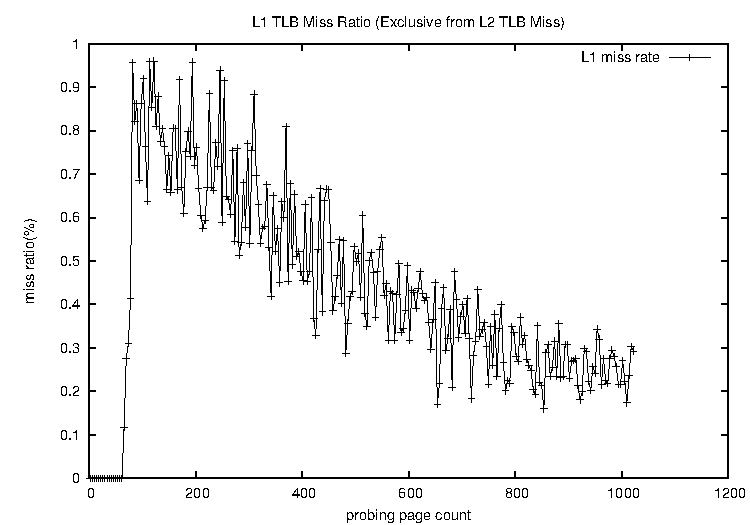
\includegraphics[width=0.9\linewidth]{../figures/tlb}
\caption{L1 TLB miss rate during memory walk, generated by \emph{perf}. The L2 TLB data, however, nearly have no missing all the time no matter how much I used the memory.
}
\label{fig:tlbsz-tlb}
\end{figure}

\begin{figure}[htp]
\centering
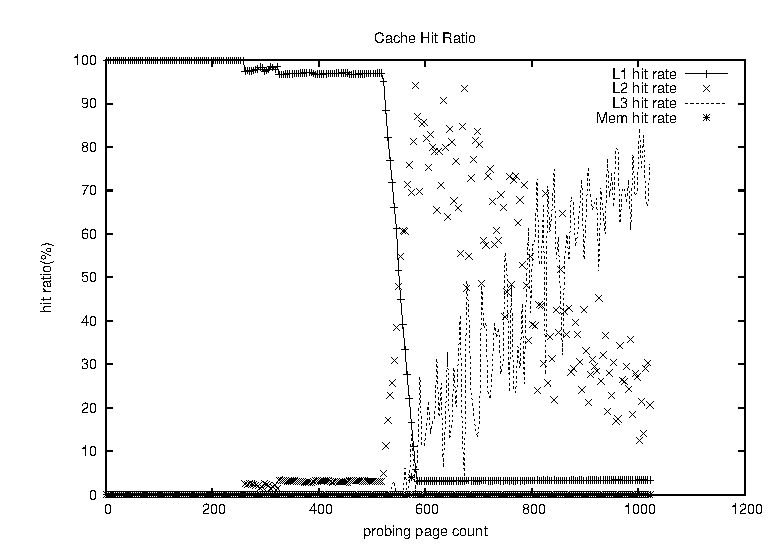
\includegraphics[width=0.9\linewidth]{../figures/cache}
\caption{Multiple level of caches hit ratio. The hit rate for each level is exclusive, i.e. if L2 cache is hit, then L1, L3 miss is not hit. Memory hit simply means memory reference, and this seldom happens}
\label{fig:tlbsz-cache}
\end{figure}

To verify the case, I use \emph{perf} to collect the hardware data. The detail
command and event used will be disclosed in appendix~\ref{append:a}. It can
also be found in~\ref{intel-dev3}.

From the figure~\ref{fig:tlbsz-cache} and figure~\ref{fig:tlbsz-tlb}, I can
confirm before the page number grows to 512, things tend to be correct, and the
L1 TLB size would be around 64 entries. However, after I reached about 512
pages, it becomes quite unstable. The reason can be found mainly in
figure~\ref{fig:tlbsz-cache}, the L2 cache begins to miss heavily.  The reason
is pages may be non-continuous in physical. I will discuss the in
section~\ref{subsec:tlb-discus}. Besides, \emph{perf} merely shows me the reasonable
L2 TLB miss number, but from the change of L1 TLB miss rate, which means L1 TLB
miss and L2 TLB hit, it can be seen that L2 TLB is missing, just that performance
counter does not read correct number. It could be buggy implementations in perf or
I could misuse the command, and the reason for this is not resolved yet.

\subsection{Discussion}
\label{subsec:tlb-discus}
The first time I used register-base-scale addressing to implement the walk
kernel. However, this is not quite good choice. The reason is even CPU miss
on a TLB visit, it can still issue following instructions because there are
no data dependency, and the overhead is ammortized so that phase change is
not clear, even if I have observed high TLB miss rate and cache hit rate.

The next method I tried is using linked list. In each cache line I encode the
next address to visit and make it a linked list. In this way, the phase change
become apparent when I increase the probing page count by factor 2. However, if
I increase probing count 1 by 1, then the normalized time for one memory
reference exhibits the above behavior. The reason to blame for is the potential
of non-continuous physical page. On my platform, there will be 512 cache sets
on L2 cache, which means, if using 4KB page, 3 higher bit used to reference
the cache sets will not be controllable by users. Operating system can even
enforce the cache separation by not allocating physical pages with certain
set index to users. The problem here is, although in theory we could probe
more than 4096 (8-way 512 sets) pages before L2 cache misses, in practice
only 512 (8-way and 6-bit sets) can be ensured to visit without miss.

An interesting observation is the chance for 8 pages having same high 3-bit
index is rare. So we can adjust the walking algorithm, rather than fixing the
stride and period of walking, we probe the good page sets, i.e. those uniformly
distributed over the bits [15:12], this can be observed from timing result
again. In such way, when we found enough pages, we can go on our walk by linking
these pages together. I haven't got time to derive the actual expectation, but
it should be much larger than the current turning point 512.

In my experiments, I didn't measure the size of huge page TLB. One reason is it
is developing toward unified TLB, which measuring the small page TLB is enough.
On the other hand, the whole thing required to measure huge TLB would be similar
as above process, and much easier since L2 cache sets will all be embodied inside
the continuous huge pages.

